\documentclass[]{article}

\usepackage[nonatbib,preprint]{neurips}

\usepackage[utf8]{inputenc} % allow utf-8 input
\usepackage[T1]{fontenc}    % use 8-bit T1 fonts
\usepackage{hyperref}       % hyperlinks
\usepackage{url}            % simple URL typesetting
\usepackage{booktabs}       % professional-quality tables
\usepackage{amsfonts}       % blackboard math symbols
\usepackage{nicefrac}       % compact symbols for 1/2, etc.
\usepackage{microtype}      % microtypography
\usepackage{graphicx}
\usepackage{caption}
\usepackage{subcaption}
\usepackage{pgffor} % for loop
\usepackage{xstring} % for declaring lists



\graphicspath{{../figures/example-figures/}}


\title{Generalisation report}

\author{%
	Generalisation report produced by \href{https://github.com/bethgelab/model-vs-human}{model-vs-human}\\
}



\begin{document}

\newcommand{\figwidth}{0.24\textwidth}
\newcommand{\captionspace}{-1.5\baselineskip}
\newcommand{\captionspaceII}{0.6\baselineskip}
\newcommand{\captionspaceBenchmark}{-0.5\baselineskip}


\maketitle

%\begin{abstract}
%\end{abstract}


\begin{figure}[h]
	\begin{subfigure}{0.49\linewidth}
		\centering
		\includegraphics[width=\linewidth]{benchmark_16-class-accuracy.pdf}
		%\vspace{\captionspaceBenchmark}
		\caption{OOD accuracy (higher = better).}
		\label{subfig:benchmark_a}
		\vspace{\captionspaceII}
	\end{subfigure}\hfill
	\begin{subfigure}{0.49\linewidth}
		\centering
		\includegraphics[width=\linewidth]{benchmark_16-class-accuracy-difference.pdf}
		%\vspace{\captionspaceBenchmark}
		\caption{Accuracy difference (lower = better).}
		\label{subfig:benchmark_b}
		\vspace{\captionspaceII}
	\end{subfigure}\hfill
	\begin{subfigure}{0.49\linewidth}
		\centering
		\includegraphics[width=\linewidth]{benchmark_observed-consistency.pdf}
		%\vspace{\captionspaceBenchmark}
		\caption{Observed consistency (higher = better).}			\label{subfig:benchmark_c}
		\vspace{\captionspaceII}
	\end{subfigure}\hfill
	\begin{subfigure}{0.49\linewidth}
		\centering
		\includegraphics[width=\linewidth]{benchmark_error-consistency.pdf}
		%\vspace{\captionspaceBenchmark}
		\caption{Error consistency (higher = better).}			\label{subfig:benchmark_d}
		\vspace{\captionspaceII}
	\end{subfigure}\hfill
	\caption{Benchmark results for different models, aggregated over datasets.}
	\label{fig:benchmark_barplots}
\end{figure}

\begin{table}[ht]
	\caption{Benchmark table of model results for most human-like behaviour. The three metrics ``accuracy difference'' ``observed consistency'' and ``error consistency'' (plotted in Figure~\ref{fig:benchmark_barplots}) each produce a different model ranking. The mean rank of a model across those three metrics is used to rank the models on our benchmark.}
	\label{tab:benchmark_table_humanlike}
	\centering
	\begin{tabular}{lrrrr}
\toprule
    model & accuracy diff. $\downarrow$ & obs. consistency $\uparrow$ & error consistency $\uparrow$ & mean rank $\downarrow$ \\
\midrule
SimCLR-x1 &              \textbf{0.080} &              \textbf{0.667} &                        0.179 &         \textbf{1.333} \\
ResNet-50 &                       0.087 &                       0.665 &               \textbf{0.208} &                  1.667 \\
BagNet-33 &                       0.156 &                       0.567 &                        0.137 &                  3.000 \\
\bottomrule
\end{tabular}


\end{table}

\begin{table}[h!]
	\caption{Benchmark table of model results for highest out-of-distribution robustness.}
	\label{tab:benchmark_table_accurate}
	\centering
	\begin{tabular}{lrr}
\toprule
    model & OOD accuracy $\uparrow$ & rank $\downarrow$ \\
\midrule
SimCLR-x1 &          \textbf{0.596} &    \textbf{1.000} \\
ResNet-50 &                   0.559 &             2.000 \\
BagNet-33 &                   0.398 &             3.000 \\
\bottomrule
\end{tabular}


\end{table}



\begin{figure}
	%	% colour vs. greyscale | true vs. false colour
	\begin{subfigure}{\figwidth}
			\centering
			\textbf{Accuracy}\\
			\includegraphics[width=\linewidth]{colour_OOD-accuracy.pdf}
			\vspace{\captionspace}
			\caption{Colour vs. greyscale}
			\vspace{\captionspaceII}
		\end{subfigure}\hfill
		\begin{subfigure}{\figwidth}
			\centering
			\textbf{Error consistency}\\
			\includegraphics[width=\linewidth]{colour_error-consistency.pdf}
			\vspace{\captionspace}
			\caption*{}
			\vspace{\captionspaceII}
		\end{subfigure}\hfill
		\begin{subfigure}{\figwidth}
			\centering
			\textbf{Accuracy}\\
			\includegraphics[width=\linewidth]{false-colour_OOD-accuracy.pdf}
			\vspace{\captionspace}
			\caption{True vs. false colour}
			\vspace{\captionspaceII}
		\end{subfigure}\hfill
		\begin{subfigure}{\figwidth}
			\centering
			\textbf{Error consistency}\\
			\includegraphics[width=\linewidth]{false-colour_error-consistency.pdf}
			\vspace{\captionspace}
			\caption*{}
			\vspace{\captionspaceII}
		\end{subfigure}\hfill
	
	% uniform noise | low pass
		\begin{subfigure}{\figwidth}
			\centering
			\includegraphics[width=\linewidth]{uniform-noise_OOD-accuracy.pdf}
			\vspace{\captionspace}
			\caption{Uniform noise}
			\vspace{\captionspaceII}
		\end{subfigure}\hfill
		\begin{subfigure}{\figwidth}
			\centering
			\includegraphics[width=\linewidth]{uniform-noise_error-consistency.pdf}
			\vspace{\captionspace}
			\caption*{}
			\vspace{\captionspaceII}
		\end{subfigure}\hfill
		\begin{subfigure}{\figwidth}
			\centering
			\includegraphics[width=\linewidth]{low-pass_OOD-accuracy.pdf}
			\vspace{\captionspace}
			\caption{Low-pass}
			\vspace{\captionspaceII}
		\end{subfigure}\hfill
		\begin{subfigure}{\figwidth}
			\centering
			\includegraphics[width=\linewidth]{low-pass_error-consistency.pdf}
			\vspace{\captionspace}
			\caption*{}
			\vspace{\captionspaceII}
		\end{subfigure}\hfill
		
	%	% contrast | high-pass
		\begin{subfigure}{\figwidth}
			\centering
			\includegraphics[width=\linewidth]{contrast_OOD-accuracy.pdf}
			\vspace{\captionspace}
			\caption{Contrast}
			\vspace{\captionspaceII}
		\end{subfigure}\hfill
		\begin{subfigure}{\figwidth}
			\centering
			\includegraphics[width=\linewidth]{contrast_error-consistency.pdf}
			\vspace{\captionspace}
			\caption*{}
			\vspace{\captionspaceII}
		\end{subfigure}\hfill
		\begin{subfigure}{\figwidth}
			\centering
			\includegraphics[width=\linewidth]{high-pass_OOD-accuracy.pdf}
			\vspace{\captionspace}
			\caption{High-pass}
			\vspace{\captionspaceII}
		\end{subfigure}\hfill
		\begin{subfigure}{\figwidth}
			\centering
			\includegraphics[width=\linewidth]{high-pass_error-consistency.pdf}
			\vspace{\captionspace}
			\caption*{}
			\vspace{\captionspaceII}
		\end{subfigure}\hfill
	
	    % eidolon I | phase noise
		\begin{subfigure}{\figwidth}
			\centering
			\includegraphics[width=\linewidth]{eidolonI_OOD-accuracy.pdf}
			\vspace{\captionspace}
			\caption{Eidolon I}
			\vspace{\captionspaceII}
		\end{subfigure}\hfill
		\begin{subfigure}{\figwidth}
			\centering        \includegraphics[width=\linewidth]{eidolonI_error-consistency.pdf}
			\vspace{\captionspace}
			\caption*{}
			\vspace{\captionspaceII}
		\end{subfigure}\hfill
		\begin{subfigure}{\figwidth}
			\centering
			\includegraphics[width=\linewidth]{phase-scrambling_OOD-accuracy.pdf}
			\vspace{\captionspace}
			\caption{Phase noise}
			\vspace{\captionspaceII}
		\end{subfigure}\hfill
		\begin{subfigure}{\figwidth}
			\centering
			\includegraphics[width=\linewidth]{phase-scrambling_error-consistency.pdf}
			\vspace{\captionspace}
			\caption*{}
			\vspace{\captionspaceII}
		\end{subfigure}\hfill
		
	%	eidolon II | power equalisation
	\begin{subfigure}{\figwidth}
		\centering
		\includegraphics[width=\linewidth]{eidolonII_OOD-accuracy.pdf}
		\vspace{\captionspace}
		\caption{Eidolon II}
		\vspace{\captionspaceII}
	\end{subfigure}\hfill
	\begin{subfigure}{\figwidth}
		\centering
		\includegraphics[width=\linewidth]{eidolonII_error-consistency.pdf}
		\vspace{\captionspace}
		\caption*{}
		\vspace{\captionspaceII}
	\end{subfigure}\hfill
	\begin{subfigure}{\figwidth}
		\centering
		\includegraphics[width=\linewidth]{power-equalisation_OOD-accuracy.pdf}
		\vspace{\captionspace}
		\caption{Power equalisation}
		\vspace{\captionspaceII}
	\end{subfigure}\hfill
	\begin{subfigure}{\figwidth}
		\centering
		\includegraphics[width=\linewidth]{power-equalisation_error-consistency.pdf}
		\vspace{\captionspace}
		\caption*{}
		\vspace{\captionspaceII}
	\end{subfigure}\hfill
	
	% eidolon III | rotation
	\begin{subfigure}{\figwidth}
		\centering
		\includegraphics[width=\linewidth]{eidolonIII_OOD-accuracy.pdf}
		\vspace{\captionspace}
		\caption{Eidolon III}
	\end{subfigure}\hfill
	\begin{subfigure}{\figwidth}
		\centering        \includegraphics[width=\linewidth]{eidolonIII_error-consistency.pdf}
		\vspace{\captionspace}
		\caption*{}
	\end{subfigure}\hfill
	\begin{subfigure}{\figwidth}
		\centering
		\includegraphics[width=\linewidth]{rotation_OOD-accuracy.pdf}
		\vspace{\captionspace}
		\caption{Rotation}
	\end{subfigure}\hfill
	\begin{subfigure}{\figwidth}
		\centering
		\includegraphics[width=\linewidth]{rotation_error-consistency.pdf}
		\vspace{\captionspace}
		\caption*{}
	\end{subfigure}\hfill
	\caption{OOD accuracy and error consistency.}
	\label{fig:results_accuracy_error_consistency}
\end{figure}
\begin{figure}[h]
	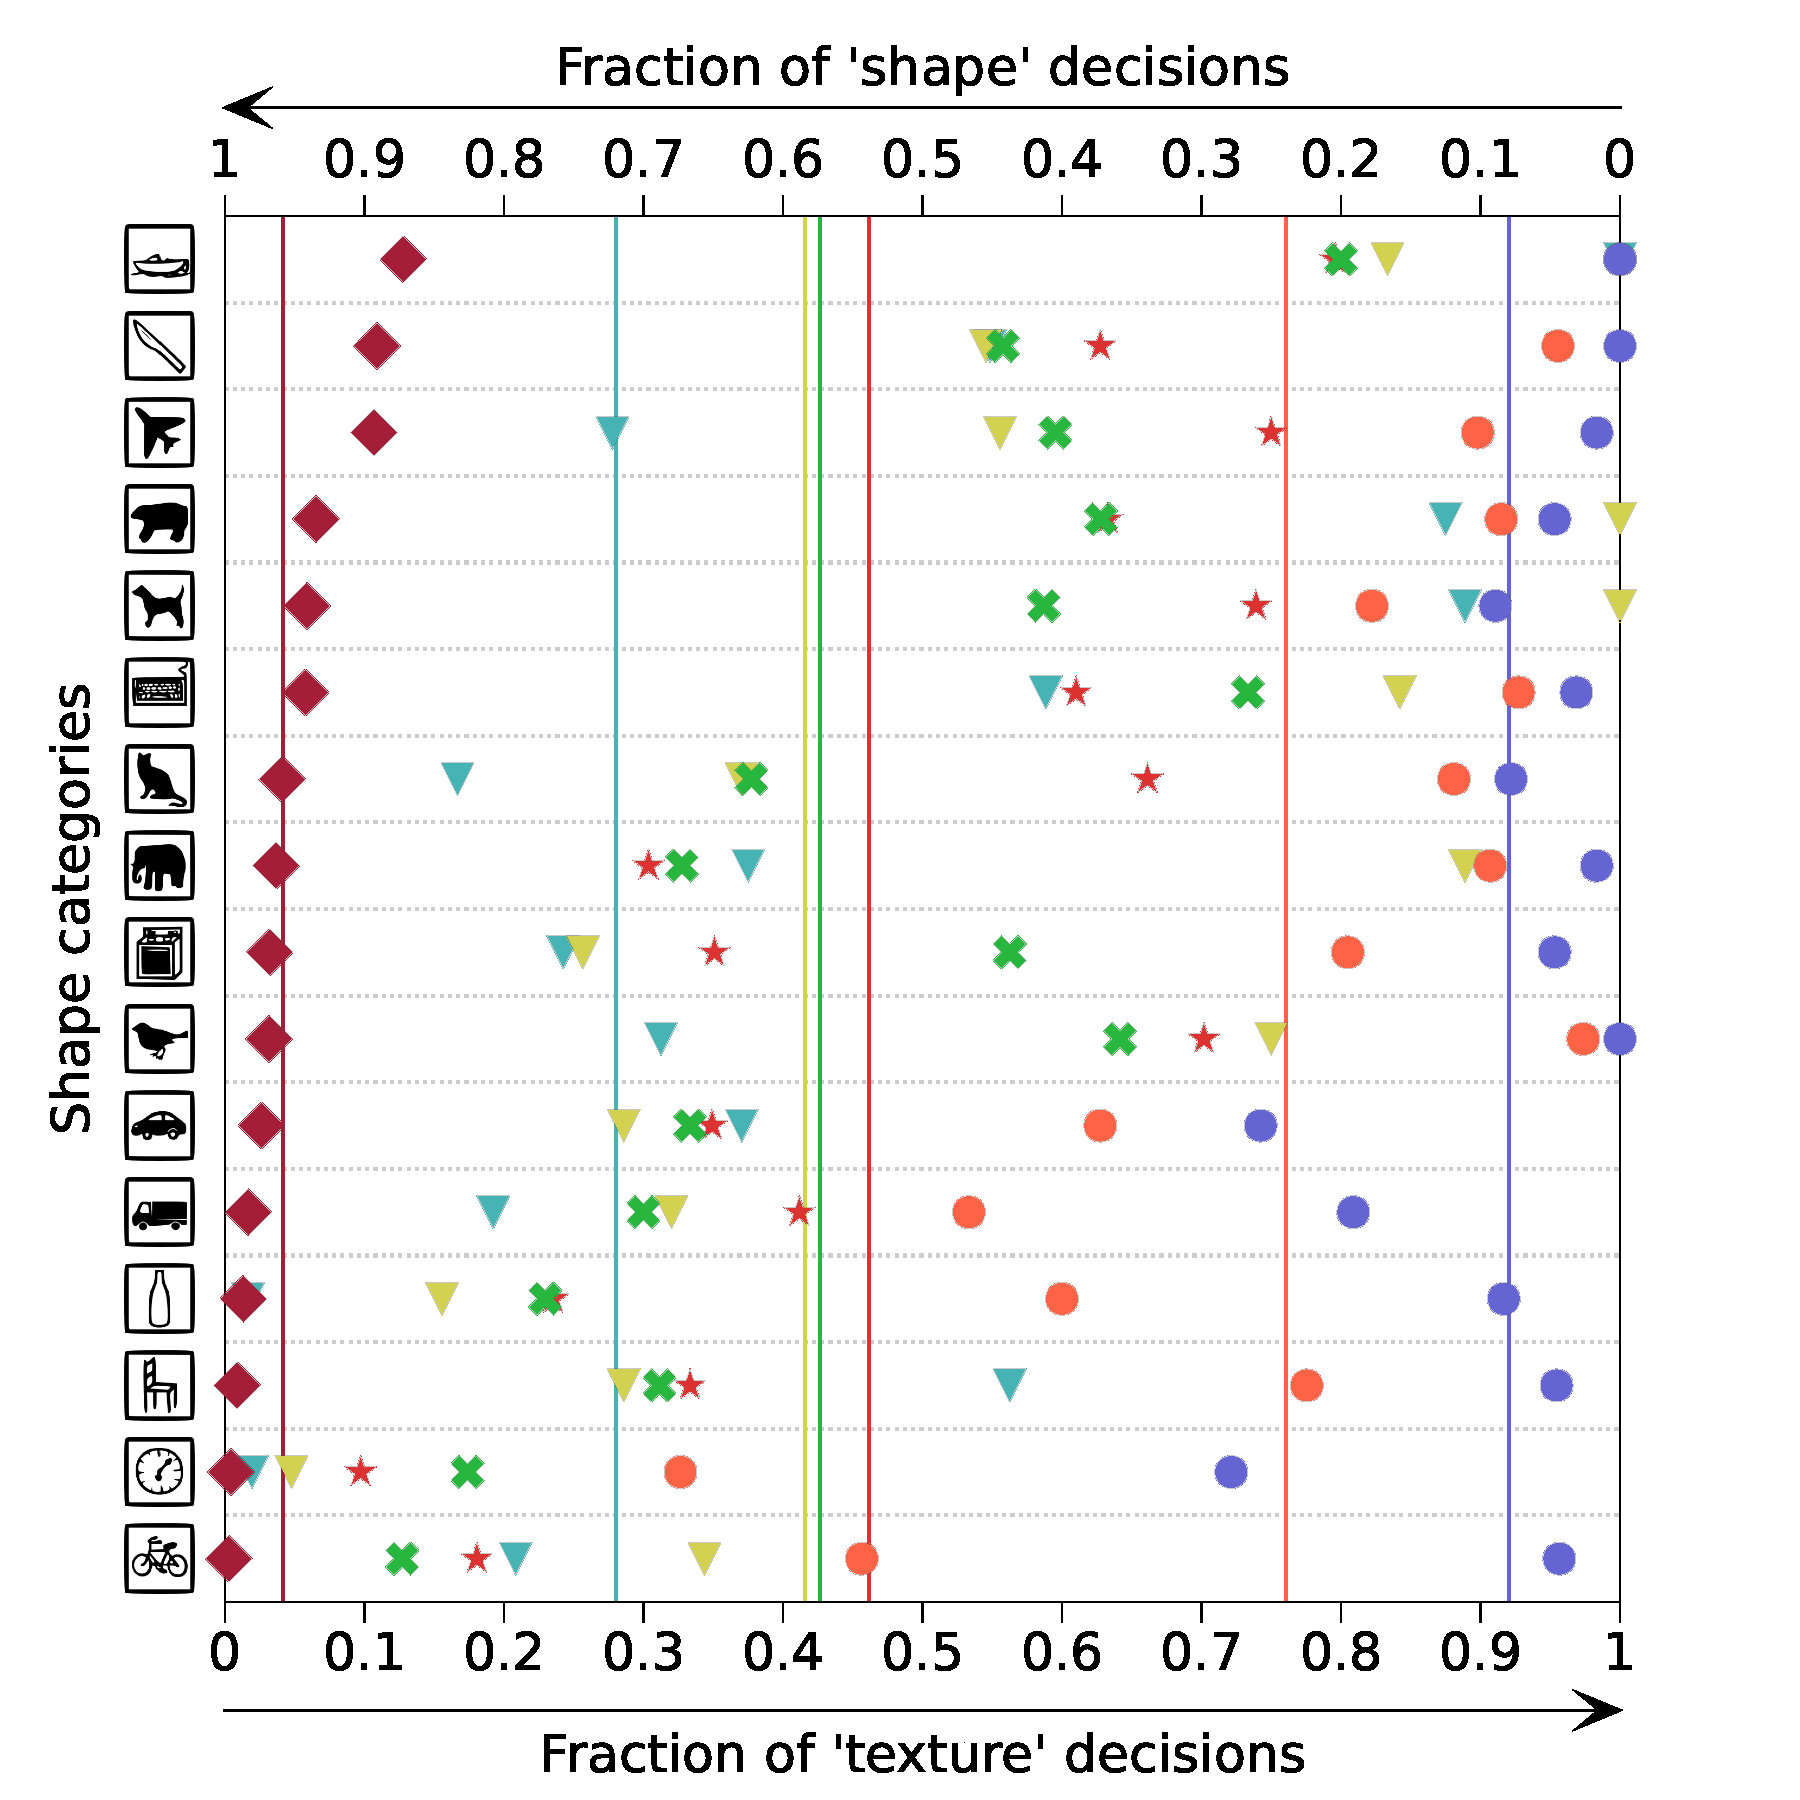
\includegraphics[width=\linewidth]{cue-conflict_shape-bias_matrixplot.pdf}
	\caption{Shape vs.\ texture bias: category-level plot.}
\end{figure}\hfill


\begin{figure}[h]
	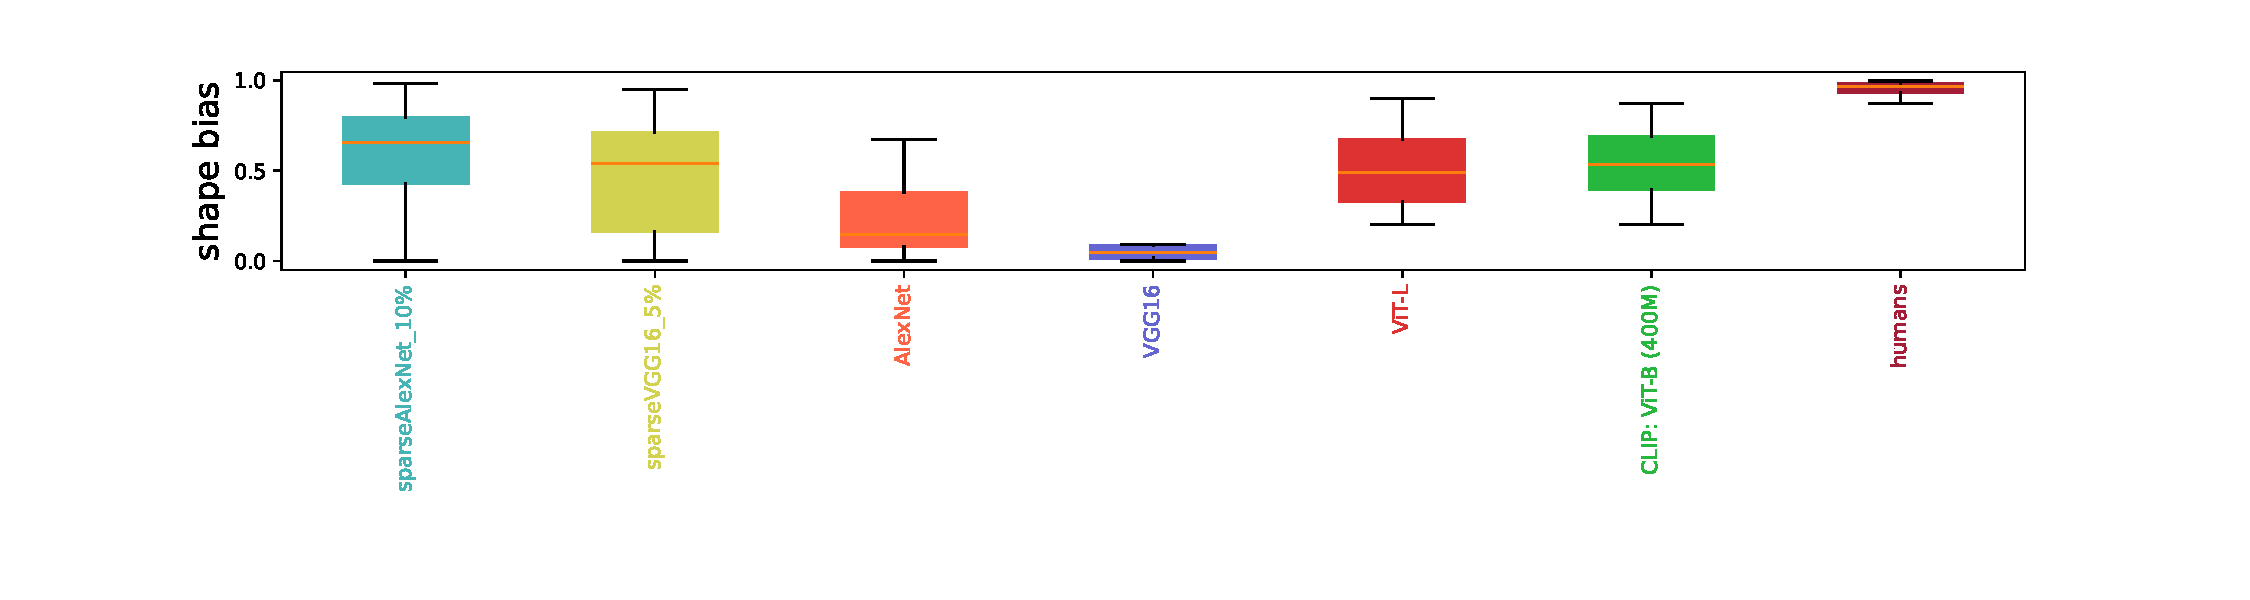
\includegraphics[width=\linewidth]{cue-conflict_shape-bias_boxplot.pdf}
	\caption{Shape vs.\ texture bias: boxplot.}
\end{figure}\hfill

\begin{figure}[h]
    \centering
    \begin{subfigure}{0.45\textwidth}
        \centering
        \includegraphics[width=\linewidth]{scatter-plot_OOD-accuracy_vs_observed-consistency_multiple-datasets.pdf}
        %\vspace{-0.1cm}
        \caption{Out-of-distribution accuracy vs.\\observed consistency}
        \label{subfig:error_consistency_12_datasets}
    \end{subfigure}
    \begin{subfigure}{0.45\textwidth}
        \centering
        \includegraphics[width=\linewidth]{scatter-plot_OOD-accuracy_vs_error-consistency_multiple-datasets.pdf}
        %\vspace{-0.1cm}
        \caption{Out-of-distribution accuracy vs.\\error consistency}
        \label{subfig:error_consistency_5_datasets}
    \end{subfigure}
    \label{fig:error_consistency_12_and_5_datasets}
    \vspace{-0.1cm}
    \caption{Observed consistency and error consistency between models and humans as a function of out-of-distribution (OOD) accuracy. Dotted lines indicate consistency expected by chance.}
\end{figure}
\begin{figure}
	\centering
	\includegraphics[width=0.8\linewidth]{sketch_error-consistency_matrix.pdf}
	\caption{Error consistency for `sketch' images.}
	\label{fig:error_consistency_matrix_sketch}
\end{figure}

\begin{figure}
    \centering
    \includegraphics[width=0.8\linewidth]{stylized_error-consistency_matrix.pdf}
    \caption{Error consistency for `stylized' images.}
    \label{fig:error_consistency_matrix_stylized}
\end{figure}

\begin{figure}
	\centering
	\includegraphics[width=0.8\linewidth]{edge_error-consistency_matrix.pdf}
	\caption{Error consistency for `edge' images.}
	\label{fig:error_consistency_matrix_edges}
\end{figure}

\begin{figure}
	\centering
	\includegraphics[width=0.8\linewidth]{silhouette_error-consistency_matrix.pdf}
	\caption{Error consistency for `silhouette' images.}
	\label{fig:error_consistency_matrix_silhouettes}
\end{figure}

\begin{figure}
	\centering
	\includegraphics[width=0.8\linewidth]{cue-conflict_error-consistency_matrix.pdf}
	\caption{Error consistency for `cue conflict' images.}
	\label{fig:error_consistency_matrix_cue-conflict}
\end{figure}





\end{document}
